% [beamer を使うために] by J.Goto (Jul.14,2008+Nov.03,2011)
%
% 0. まず, TeXがインストールされていることが前提となります. 
%    TeXがインストールされていない場合は, まずTeX(pLaTeXなど)をインストールして下さい。
% 1. 次に, https://sourceforge.net/projects/latex-beamer/ から必要なファイルをダウンロード&展開します.
%    とりあえず, latex-beamer, pgf, xcolor(フォルダ)をダウンロードして, 
%    適当な場所に適当なファイル解凍ソフトで展開します.
%
%    ## 2011年11月3日現在、上記にあるヴァージョンはやや古いようです。
%    ## 上記のものではなく、下記のダウンロード先を参照してみてください。
%    ## 【beamer本体】http://www.ctan.org/tex-archive/macros/latex/contrib/beamer/
%    ## 【pgf】       http://sourceforge.net/projects/pgf/files/pgf/version%202.00/pgf-2.00.tar.gz/download
%    ## 【xcolor】    http://www.ctan.org/tex-archive/macros/latex/contrib/xcolor/
%
% 2. 展開されたlatex-beamer, pgf, xcolorの3つのフォルダを適当なフォルダ(/texmf/tex/latex/)に置きます. 
%    詳しくは http://sourceforge.net/docman/display_doc.php?docid=19464&group_id=92412 を参照して下さい.
%    ちなみに, 僕の場合は, TeXがインストールされているフォルダを/tex/とすると, 
%    /tex/share/texmf/tex/latex/に3つのフォルダを置きました.
% 3. 後はTeXと同じように.texファイルを作成し, コンパイルして使います. 
%    もちろん, クラスファイルの読み込みや, その入力ルールに従う必要があります.(以下を参考)
%
% -- beamerを初めて使うときは, これより下の部分を, 適当に置き換えながら使ってみましょう --

\documentclass[11pt,dvipdfmx]{beamer}

%%% 使用するテーマ(現在Copenhagenを指定しています。適当に変えてみよう。)%%%
%
\usetheme{Antibes}  
%\usetheme{Default}       % シンプルで機能的なテーマ #何も指定しない場合は自動的にこれ
%\usetheme{Bergen}        % フレームを縦方向に分割
%\usetheme{Boadilla}      % より多くの情報を収容可
%\usetheme{Madrid}        % Boadillaをよりカラフルにしたもの
%\usetheme{Pittsburgh}    % シンプルで機能的、見出しは右寄せ
%\usetheme{Rochester}     % 横方向のヘッダパネルが特徴     % 上部にナビゲーションバーを持つ、明瞭度の高いテーマ
%\usetheme{JuanLesPins}   % Antibesと類似のテーマ
%\usetheme{Montpellier}   % シンプルで色調のおとなしいもの
%\usetheme{Berkeley}      % 横方向のヘッダパネルを持つ機能的なテーマ
%\usetheme{PaloAlto}      % Berkeleyと類似のテーマ
%\usetheme{Goettingen}    % サイドバーは右側で、ヘッダパネルなし
%\usetheme{Marburg}       % Goettingenの色調を強くしたもの
%\usetheme{Hannover}      % サイドバーは左側で見出しは右寄せ
%\usetheme{Berlin}        % 縦方向のナビゲーションバーを上部に持つ強い色調のテーマ
%\usetheme{Ilmenau}       % Berlinと類似のテーマ
%\usetheme{Dresden}       % Ilmenauと類似のテーマ
%\usetheme{Darmstadt}     % 横方向のナビゲーションバーを上部に持つ
%\usetheme{Frankfurt}     % Darmstadtと類似、しかしサブセクション情報は含まない
%\usetheme{Singapore}     % ソフトな色調を持ったテーマ
%\usetheme{Szeged}        % Singaporeと類似、しかし境界線は明確
%\usetheme{Copenhagen}    % セクション/サブセクションテーブルを上部に配置
%\usetheme{Luebeck}       % Copenhagenから丸みを取ったもの
%\usetheme{Malmoe}        % Copenhagenをより質素にしたもの
\usetheme{Warsaw}        % Copenhagenと類似のテーマ

%%% 数式のフォント(TeXっぽいフォントになる)%%%
%
\usefonttheme{professionalfonts}


%%% 隠蔽されている要素の透明度の設定 %%%
%
%\setbeamercovered{transparent=10}

%%% その他のクラス・パッケージの導入 %%%

\usepackage{graphicx}  % includegraphicsコマンドなどで図を表示するためのクラス
\usepackage{amsmath}   % プロ仕様の数学用のフォントI(AMSはアメリカ数学会)
\usepackage{amssymb}   % プロ仕様の数学用のフォントII(AMSはアメリカ数学会)
\usepackage{bm}        % 太字を表現するのに便利なクラス
\usepackage[absolute,overlay]{textpos}


\usepackage[all]{xy}
\usepackage{amsthm,amsmath,amssymb,comment}
\usepackage{float}
\usepackage{graphicx}
%% ゴシック体にする
%\renewcommand{\kanjifamilydefault}{gt}

% フォントはお好みで
%\usepackage{txfonts}
%\mathversion{bold}                             %%% 数式を太字にする
\renewcommand{\familydefault}{\sfdefault}
\renewcommand{\kanjifamilydefault}{\gtdefault} %%% 日本語フォントを太字にする
%\setbeamerfont{title}{size=\large,series=\bfseries}
%\setbeamerfont{frametitle}{size=\large,series=\bfseries}
%\setbeamertemplate{frametitle}[default][center]
%\usefonttheme{professionalfonts} 
%
\newtheorem{proposition}{命題}
\newtheorem{assumption}{仮定}
\newtheorem{cor}{系}
\newtheorem{remark}{Remark}
\newtheorem{exercise}{Exercise}

\newtheorem{thm}{Theorem}[section] 
\newtheorem{theo}[thm]{Theorem}
\newtheorem{corr}[thm]{Corollary}
\newtheorem{prop}[thm]{Proposition}
\newtheorem{conj}[thm]{Conjecture}
\newtheorem*{mainthm}{Theorem}
\newtheorem{deflem}[thm]{Definition-Lemma}
\newtheorem{lem}[thm]{Lemma}
\theoremstyle{definition} 
\newtheorem{defn}[thm]{Definition}
\newtheorem{propdefn}[thm]{Proposition-Definition} 
\newtheorem{lemdefn}[thm]{Lemma-Definition} 
\newtheorem{thmdefn}[thm]{Theorem-Definition} 
\newtheorem{eg}[thm]{Example} 
\newtheorem{ex}[thm]{Example} 
\theoremstyle{remark}
\newtheorem{rem}[thm]{Remark}
\newtheorem{obs}[thm]{Observation}
\newtheorem{ques}[thm]{Question}
%\newtheorem{problem}[thm]{Problem}
\newtheorem{setup}[thm]{Set up}
\newtheorem{notation}[thm]{Notation}
\newtheorem{cl}{Claim}
\newtheorem{claim}{Claim}
\newtheorem{step}{Step}
\newtheorem*{clproof}{Proof of Claim}
\newtheorem{cln}[thm]{Claim}
\newtheorem*{ack}{Acknowledgements} 



%% 自分で定義したマクロ
\newcommand{\Sym}{{\rm Sym}}

\newcommand{\Sigmat}{\mbox{\boldmath\ensuremath{\Sigma}}}
\newcommand{\evec}{\mbox{\boldmath\ensuremath{e}}}
\newcommand{\ovec}{\mbox{\boldmath\ensuremath{0}}}
\newcommand{\xvec}{\mbox{\boldmath\ensuremath{x}}}
\newcommand{\R}{{\rm I\!R}}
\newcommand{\e}{{\rm e}}
\newcommand{\dr}{{\rm d}}
\newcommand{\E}{{\mathbb E}}
\newcommand{\p}{{\mathbb P}}
\newcommand{\V}{{\mathbb V}}


\title[2021年度前期 全学共通科目 解析I TI電(都1〜28)]{大阪市立大学 2021年度前期(R3年度前期) \\ 全学共通科目 解析I TI電(都1〜28)}
\subtitle{授業の進め方・成績の付け方について}
\author[岩井雅崇]{岩井雅崇}
%% 所属の登録 \institute[所属の略称]{所属}
\institute[大阪市立大学数学研究所]{大阪市立大学数学研究所}
%% 日付
\date{2021年4月13日}  %% <- \today 命令は今日の日付を表示. 任意の日付を入れれば良い:(例)\date{2008年7月14日}

%%% 以下が本体 %%%

\begin{document}

%%%%%%%%%%%%%%%%%%%%%%%%%%%%%%%%%%%%%%%%%%%%%%%%%%%%%%%%%%%%%%%%%%%%%%%%
%%%%%%%%%%%%%%%%%%%%%%%%%%%%%%%%%%%%%%%%%%%%%%%%%%%%%%%%%%%%%%%%%%%%%%%%
%% タイトルページ出力 %%

\begin{frame}  %% <- \begin{frame} から \end{frame}までが1つの頁になると思って下さい.
 \titlepage    %% <- このコマンドで自動的に表紙のページが作成されます.
\end{frame}

% [remark]
% \begin{frame} *** \end{frame} の代わりに
% \frame { *** } としても同じです(次のページの書き方を参考にして下さい).

%%%%%%%%%%%%%%%%%%%%%%%%%%%%%%%%%%%%%%%%%%%%%%%%%%%%%%%%%%%%%%%%%%%%%%%%
%%%%%%%%%%%%%%%%%%%%%%%%%%%%%%%%%%%%%%%%%%%%%%%%%%%%%%%%%%%%%%%%%%%%%%%%
%% 目次ページ

%%\begin{frame}  %% <- この書き方でもOK.
%% \tableofcontents   %% <- このコマンド1つで自動的に目次のページが作成されます.
%%\end{frame}

%%%%%%%%%%%%%%%%%%%%%%%%%%%%%%%%%%%%%%%%%%%%%%%%%%%%%%%%%%%%%%%%%%%%%%%%
%%%%%%%%%%%%%%%%%%%%%%%%%%%%%%%%%%%%%%%%%%%%%%%%%%%%%%%%%%%%%%%%%%%%%%%%

\section{ }
\begin{frame}
\frametitle{この授業について}
 \begin{itemize}


 \item この授業は"2021年度前期 全学共通科目 解析I TI電(都1〜28)"です.
 \item 担当教官は岩井雅崇(いわいまさたか)です.
 \item この授業でやることは"1変数関数の微積分"です.
 
 \end{itemize}
\end{frame}

\begin{frame}
\frametitle{なぜ微積分や線形代数を学ぶのか?}
   \begin{alertblock}{}
  \begin{center}
応用がいっぱいある.
  \end{center}
 \end{alertblock}
 
  \begin{itemize}
  \item 微積分や線型代数とか使って, 多くの理論ができている.
  \item  何らかのシミュレーションするとき, 偏微分方程式を使うから, 微積分の知識が必要.
  \item (最近の流行の) 機械学習, 深層学習, 人工知能, AI (etc...)は微積分と行列が多く出てくる.
  {\tiny (Pythonのnumpyとか行列の記法だし...)}
 
  \end{itemize}


\end{frame}

\begin{frame}
\frametitle{授業のシラバス}

\begin{textblock*}{0.4\linewidth}(20pt, 40pt)
    \centering
    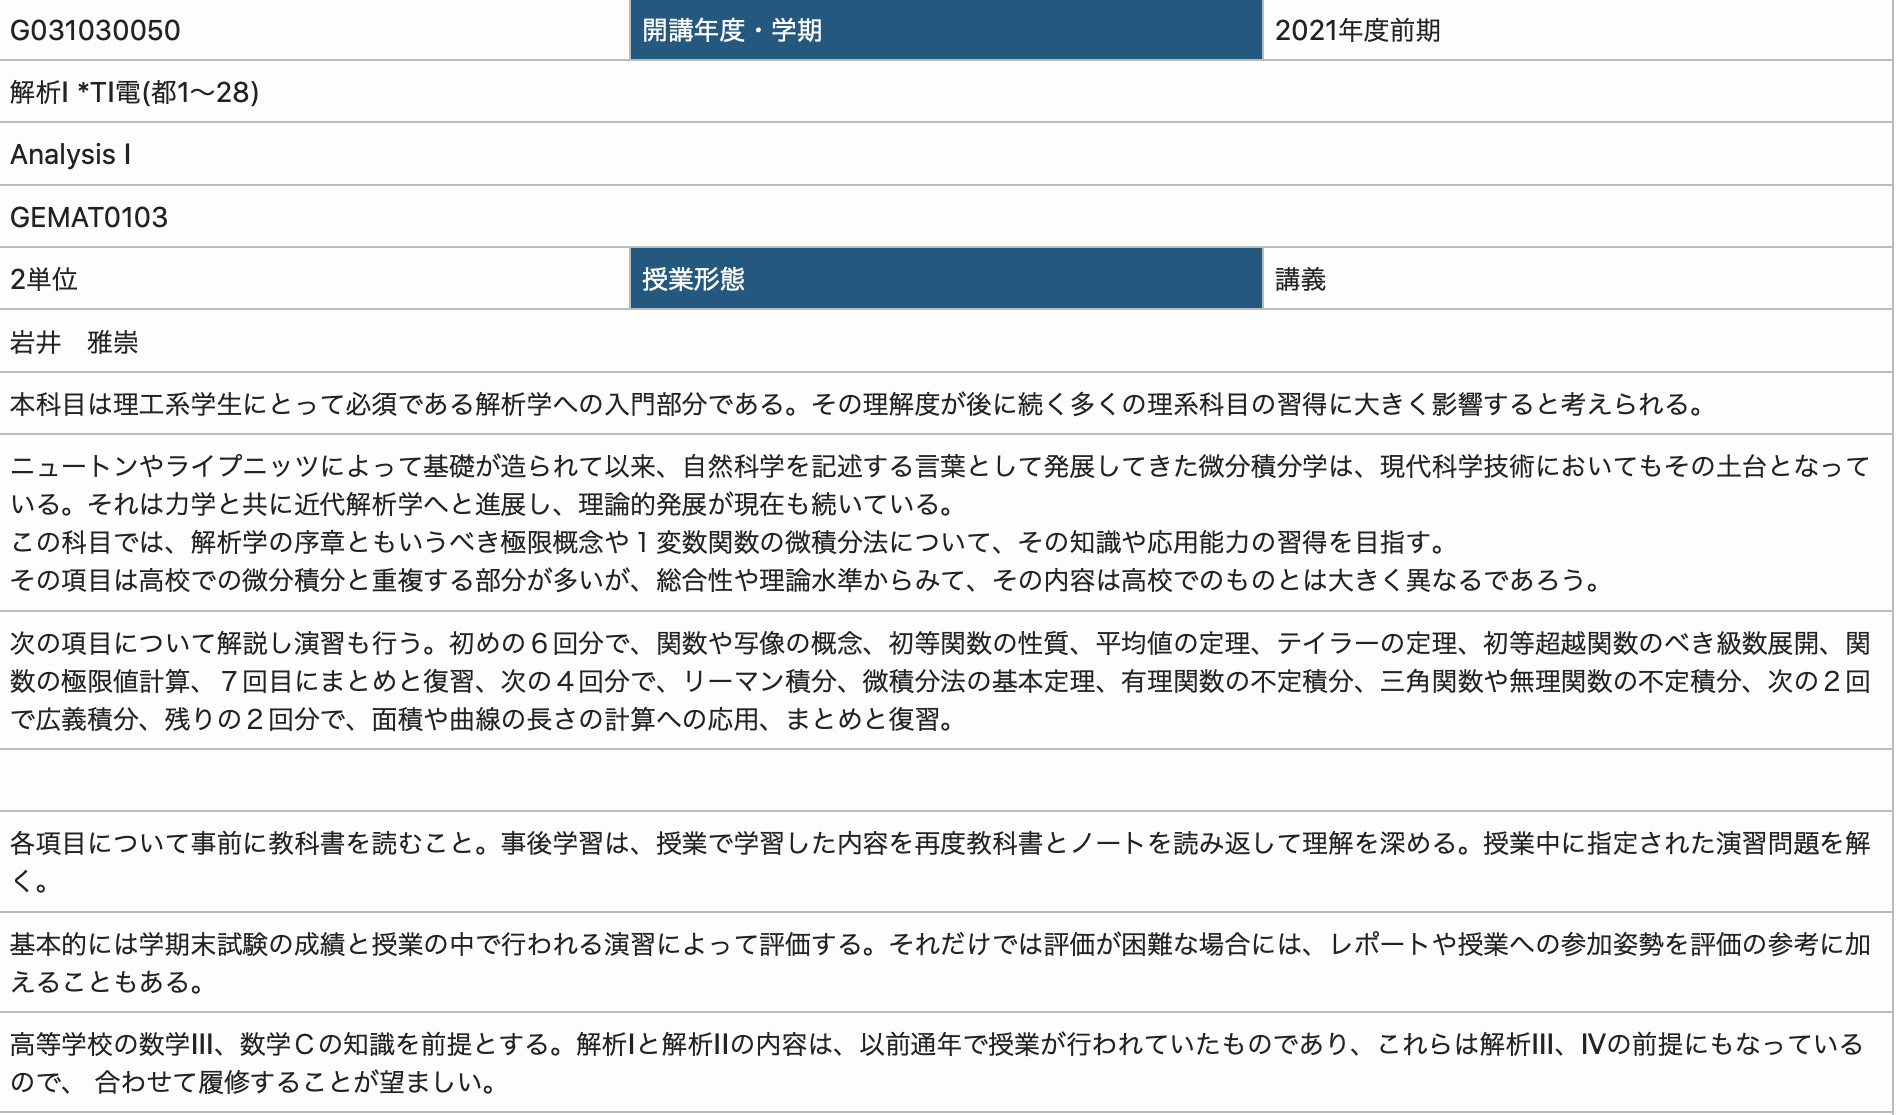
\includegraphics[height=75mm, width=110mm]{pic.jpg}
\end{textblock*}

\end{frame}

\begin{frame}
\frametitle{授業の内容}
\begin{enumerate}
\item 実数の定義と性質
\item 連続関数
\item 微分法と初等関数の性質
\item 平均値の定理と関数の極限値計算
\item 高次導関数とテイラーの定理
\item 漸近展開とべき級数展開
\item (遠隔授業の予定) まとめと復習 (予備日)
\item リーマン積分の定義と微分積分学の基本定理
\item 積分の性質 
\item 不定積分の計算方法
\item 広義積分
\item 曲線の長さ
\item (遠隔授業の予定) まとめと復習 (予備日)
\item (遠隔授業の予定) まとめと復習 (予備日)
\end{enumerate}


\end{frame}

\begin{frame}
\frametitle{成績の付け方}
 \begin{itemize}
 \item 中間レポート(50点程度)と期末試験(50点程度)のみで評価する. 
 どちらも問題は4問(小問有り)ずつである.
 \item 出席点はないので安心してください.
 %\item 合計8問(小問あり). %計120点満点. (ただし1問20点ではない)
% \item %単位が欲しいだけの人も,  全6問を解くことをお勧めします. %(かなり減点があると思うので...)
 \item (奨学金などの申請で)より良い成績がほしい方は, 上の8問に加えてレポートや試験にある"おまけ問題"(中間期末合わせて10点程度)を解いても良い. \\
 単位が欲しいだけの人は"おまけ問題"を解かなくて良い. \\
% \item 単位が欲しいだけの人は"おまけ問題"を解かなくて良い. 6問は絶対に解くこと! \\
 {\tiny 例えばレポートで79点(良)とった人がおまけ問題を正答してた場合, 成績には80点(優)つける考慮をします.
 レポートで59点(不可)とった人がおまけ問題を正答してても, 成績が60点(可)になることはない. }
{\tiny  おまけ問題を解かなくても90点以上の成績をつけることもあります.}
 \end{itemize}


\end{frame}

\begin{frame}
\frametitle{中間レポートの内容(予定)}
 \begin{itemize}
\item 微分法と初等関数の性質 (第3回)
\item 平均値の定理と関数の極限値計算 (第4回)
\item 高次導関数とテイラーの定理 (第5回)
\item 漸近展開とべき級数展開 (第6回)
 \end{itemize}
 
 おまけ問題は, 実数の定義と性質(第1回), 連続関数(第2回), 高次導関数とテイラーの定理 (第5回)の予定.
   \begin{alertblock}{}
  \begin{center}
予定なので変更の可能性もあります!
  \end{center}
 \end{alertblock}
 
 \end{frame}
 
 \begin{frame}
\frametitle{期末試験の内容(予定)}
 \begin{itemize}
\item 積分の性質 (第9回)
\item 不定積分の計算方法 (第10回)
\item 広義積分 (第11回)
 \end{itemize}
 
 おまけ問題は広義積分 (第11回)の予定.
 
   \begin{alertblock}{}
  \begin{center}
予定なので変更の可能性もあります!
  \end{center}
 \end{alertblock}
 


\end{frame}

\begin{frame}
\frametitle{授業の進め方・みなさんの学び方}
この授業は基本的に対面授業で行います. 
まとめと復習のみ遠隔授業をします.(質問タイムみたいな感じです)

%{\tiny (私の家のwifiが微弱でして.....)}
 授業ホームページに授業の資料・授業黒板の画像・授業ノート(授業原稿)をアップロードしていきます.

 \begin{alertblock}{}
  \begin{center}
学び方は皆さんにお任せします.
  \end{center}
 
 \end{alertblock}
 例えば以下の方法など挙げられます.
  \begin{itemize}
  \item 授業に出て, 私の資料や教科書で復習する.
  \item 授業に出ずに教科書を用いて勉強する. \\ (今回やるのはたった80ページの内容!)
  \item その他, 自己流で勉強する.
  \end{itemize}

  \begin{alertblock}{}
  \begin{center}
最終的にレポートや試験でだす問題を \\ 解けるぐらい理解をすればOKです.
  \end{center}
 \end{alertblock}


\end{frame}

\begin{frame}
\frametitle{最後に}
 \begin{itemize}

 \item 緊急事態宣言等々, 予期しないことで授業の形態が変わる可能性があります.
 授業ホームページはこまめにチェックしてください.
 
 
 \item  遠隔授業をする際には事前にホームページにてお知らせします.
Zoomのリンク等はWebClassでお知らせします.
 
\item 質問に関しては, メールやWebClassのメッセージでも対応いたします.
(もちろん対面での質問も可能です.)

  \begin{alertblock}{}
  \begin{center}
無理のないように自分のペースで理解をしていってください. \\
また体調が悪い場合は無理せずお休みしても構いません. \\
(出席点はないので無理する必要はございません.)
  \end{center}
 \end{alertblock}


 \end{itemize}

\end{frame}

\end{document}